\documentclass[12pt]{article}

\usepackage{graphicx}
\usepackage{geometry}
%opening
\title{Determines the distance form a point P to a segment AB}
\author{Wu Yuan Bin}

\begin{document}
	
	
	
\maketitle
Question:
Gave a 2D point P , a 2D segment AB , found the closest point Q that from P to AB ,  as shown in the figure:
\begin{figure}[t]
	\centering
	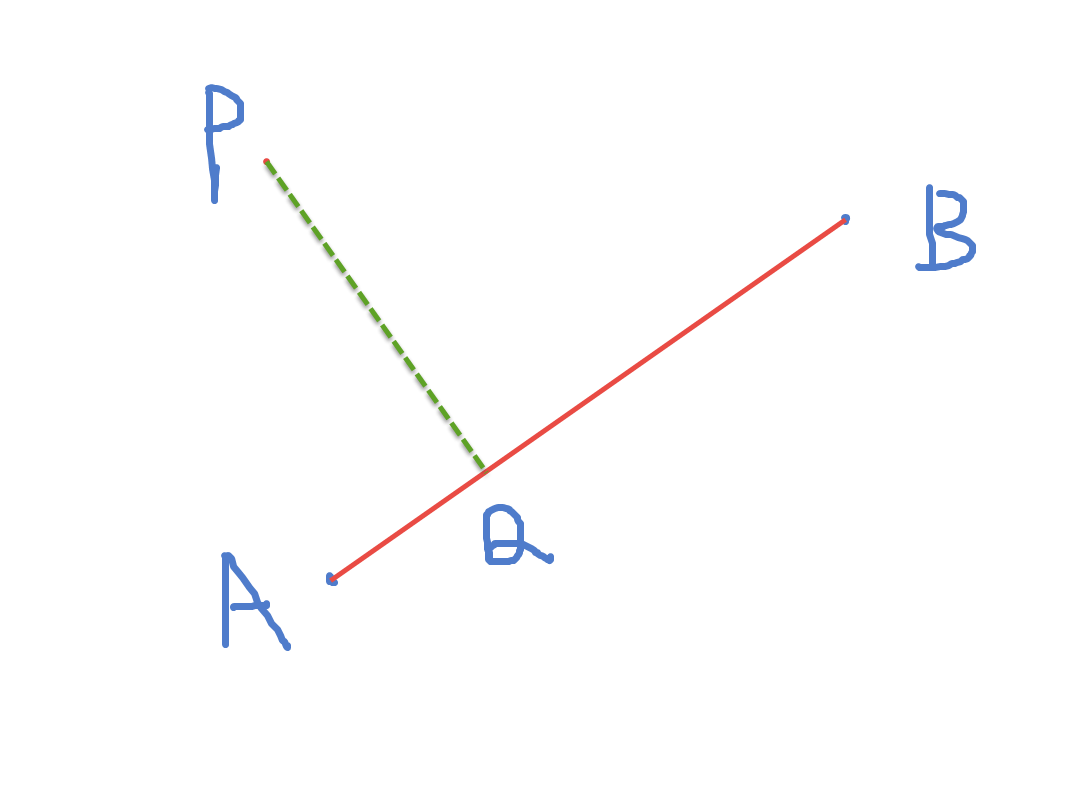
\includegraphics[width=0.5\linewidth]{pic0}
	\caption{}
	\label{fig:1}
\end{figure}\\

\section{Solution:}
\begin{enumerate}
	\item Calculate t1:
		\begin{equation}
		Q=A+(B-A)*t1
		\end{equation}
		
		\begin{eqnarray}
		A+(B-A)*t1 = P+N * d\\
		N^T *(B-A) = 0
		\end{eqnarray}
		
		BA 
		\begin{equation}
		N=\left[^{B_y-A_y}_{A_x-B_x}\right]
		\end{equation}
		
		(3) substitution (1):
		\begin{eqnarray}
		\left[^{A_x}_{A_y}\right]+\left[^{B_x-A_x}_{B_y-A_y}\right] * t1=\left[^{P_x}_{P_y}\right]+\left[^{B_y-A_y}_{A_x-B_x}\right] * d\\
		\left[^{A_x - P_x}_{A_y-P_y}\right]+\left[^{B_x-A_x}_{B_y-A_y}\right] * t1=\left[^{B_y-A_y}_{A_x-B_x}\right] * d
		\end{eqnarray}
		
		Derive:
		\begin{eqnarray}
		(A_x - P_x) + (B_x-A_x)*t1 = (B_y-A_y) * d\\
		(A_y-P_y)+(B_y-A_y) * t1 = (A_x-B_x) * d
		\end{eqnarray}
		
		Determine t1:
		\begin{equation}
		t1 = \frac{(A_y-P_y) * (B_y-A_y) - (A_x-P_x)*(A_x-B_x)}{(B_x- A_x) * (A_x - B_x)-(B_y-A_y)*(B_y - A_y)}
		\end{equation}
		
		That is :
		\begin{equation}
		t1 = \frac{(A_x-P_x)*(A_x-B_x)+(A_y-P_y) * (A_y-B_y)}{(A_x- B_x)^2+(A_y-B_y)^2}
		\end{equation}\\\\
	\item Calculate t2:
		\begin{equation}
		Q=B+(A-B)*t2
		\end{equation}
		Similarly:
		\begin{equation}
		t2 = \frac{(P_x-B_x)*(A_x-B_x)+(P_y-B_y) * (A_y-B_y)}{(A_x- B_x)^2+(A_y-B_y)^2}
		\end{equation}\\\\
	\item Conclusion:
		If $t1<=0$, the closed point from P to the segement AB is point A . So the Q = A ;\\
		If $t2 <= 0$ , the closed point from P to the segement AB is point B . So the Q = B ;\\
		Other, The Q within the segement AB,
		\begin{equation}
		Q = A + (B-A) * t
		\end{equation}
		Set: 
		\begin{eqnarray}
		a_1 = (A_x-P_x)*(A_x-B_x)+(A_y-P_y) * (A_y-B_y)\\
		a_2 = (P_x-B_x)*(A_x-B_x)+(P_y-B_y) * (A_y-B_y)
		\end{eqnarray}
		
		Follow : 
		\begin{equation}
		\vec{Q} =\vec{A} +  \frac{a_1*(\vec{B} - \vec{A})}{a_1 + a_2}
		\end{equation}
\end{enumerate}




\end{document}
